\documentclass{beamer-control}
\usepackage{beamer-control-singlefile}
\INCLUDEONLY{Linearisation}
\begin{document}
\CONCEPT{Linearisation}

\begin{SUMMARY}
\begin{itemize}
\item Jacobian Linearisation
\item Feedback Linearisation
\end{itemize}
\vfill References:
\begin{itemize}
\item \astrom{§6.4}
\end{itemize}
\end{SUMMARY}



\SUBCONCEPT{Jacobian Linearisation}

\begin{frame}{Linearisation steps}
We have nonlinear systems but can often model them linearly:
\begin{itemize}
\item Find or define equilibrium point
\item Shift coordinates so $x_e=0$
\item Make small angle approximations (e.g., $\sin\theta\approx\theta$ for $\theta\approx 0$)
\item More generally, use Taylor series expansion at the equilibrium point and truncate
\end{itemize}
\end{frame}

\begin{frame}
\frametitle{Taylor series expansion}
The Taylor series of differentiable function $f$ about point $a$ is:
\begin{align}
f(x) = f(a) + f'(a)(x - a) + \frac{f''(a)}{2!}(x - a)^2 + \cdots
\end{align}

\begin{align}
x^2 = a^2 + 2a(x - a) + (x - a)^2
\end{align}

\begin{align}
\ee^x = \sum_{n=0}^{\infty} \frac{x^n}{n!} = 1 + x + \frac{x^2}{2!} + \frac{x^3}{3!} + \cdots
\end{align}

\begin{align}
\sin(x) = \sum_{n=0}^{\infty} \frac{(-1)^n}{(2n+1)!} x^{2n+1} = x - \frac{x^3}{3!} + \frac{x^5}{5!} - \cdots
\end{align}
\end{frame}

\begin{frame}
\frametitle{Taylor series linearisation}
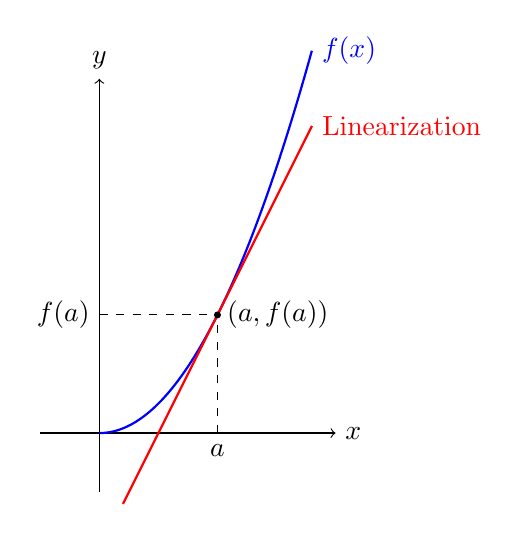
\begin{tikzpicture}[scale=1.5]

  % Axes
  \draw[->] (-0.5,0) -- (2,0) node[right] {$x$};
  \draw[->] (0,-0.5) -- (0,3) node[above] {$y$};

  % Function f(x) = x^2 (example)
  \draw[thick,blue,domain=0:1.8,smooth,samples=100] plot (\x, {\x*\x}) node[right] {$f(x)$};

  % Point a
  \def\a{1}
  \def\fa{\a*\a} % f(a) = a^2
  \def\fpa{2*\a}  % f'(a) = 2a

  % Tangent line at x = a: y = f(a) + f'(a)(x - a)
  \draw[red,thick,domain=0.2:1.8] plot (\x, {\fa + \fpa*(\x - \a)}) node[right] {Linearization};

  % Mark point (a, f(a))
  \filldraw[black] (\a, \fa) circle (0.7pt) node[right] {$(a, f(a))$};

  % Dotted lines to axes
  \draw[dashed] (\a,0) -- (\a,\fa);
  \draw[dashed] (0,\fa) -- (\a,\fa);

  % Labels
  \node at (1, -0.15) {$a$};
  \node[anchor=east] at (0, 1) {$f(a)$};

\end{tikzpicture}

\end{frame}

\begin{frame}
\frametitle{Jacobian linearisation}
The Jacobian $\frac{\partial {f}}{\partial {x}}$ is defined as a matrix of partial derivatives:
\[
{f} : \mathbb{R}^n \to \mathbb{R}^m, \quad
{f}(x_1, x_2, \ldots, x_n) = 
\begin{bmatrix}
f_1(x_1, \ldots, x_n) \\
f_2(x_1, \ldots, x_n) \\
\vdots \\
f_m(x_1, \ldots, x_n)
\end{bmatrix}
\]

\[
\frac{\partial {f}}{\partial {x}} =
\begin{bmatrix}
\frac{\partial f_1}{\partial x_1} & \frac{\partial f_1}{\partial x_2} & \cdots & \frac{\partial f_1}{\partial x_n} \\
\frac{\partial f_2}{\partial x_1} & \frac{\partial f_2}{\partial x_2} & \cdots & \frac{\partial f_2}{\partial x_n} \\
\vdots & \vdots & \ddots & \vdots \\
\frac{\partial f_m}{\partial x_1} & \frac{\partial f_m}{\partial x_2} & \cdots & \frac{\partial f_m}{\partial x_n}
\end{bmatrix}
\]

\end{frame}

\begin{frame}
\frametitle{Jacobian linearisation}
The Jacobian allows a generalised approach. For system:
\begin{align}
\dot x &= f(x,u) & y &= h(x,u)
\end{align}
Define new variables as deviation from equilibrium:
\begin{align}
z &= x - x_e & v &= u - u_e & w&= y-h(x_e,u_e)
\end{align}
Then, linearised system is:
\begin{align}
\dot z &= Az+bv & w &= Cz + Dv
\end{align}
where
\begin{align}
A &= \left.\PDeriv{f}{x}\right|_{(x_e,u_e)} &
B &= \left.\PDeriv{f}{u}\right|_{(x_e,u_e)} &
C &= \left.\PDeriv{h}{x}\right|_{(x_e,u_e)} &
D &= \left.\PDeriv{h}{u}\right|_{(x_e,u_e)}
\end{align}
\end{frame}

\begin{frame}
\frametitle{Example of Jacobian linearisation}
\centering

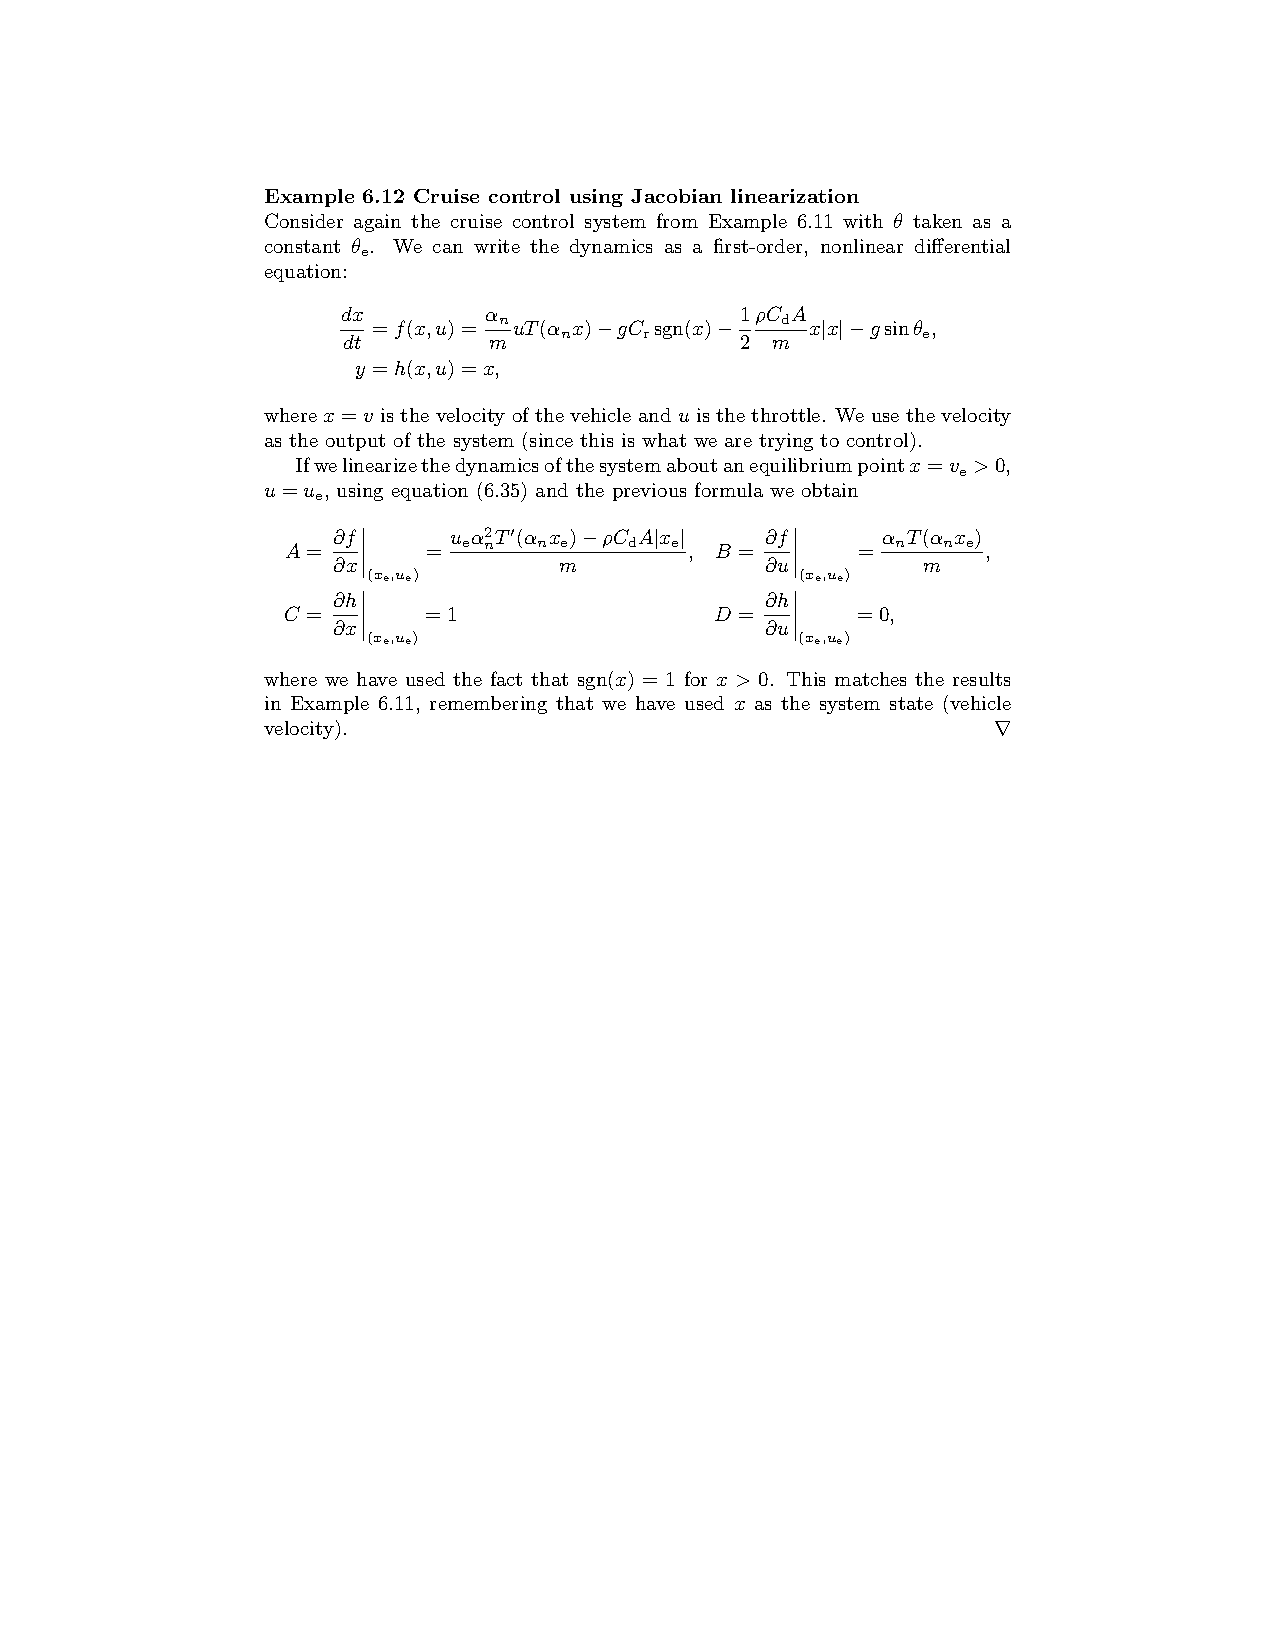
\includegraphics[height=0.8\textheight]{example6.12}

\end{frame}

\SUBCONCEPT{Feedback Linearisation}

\begin{frame}{Feedback Linearisation of quadratic term}
E.g., known nonlinearity $x^2$:
\begin{align}
\dot x &= x^2 + u &
u &= -x^2 - kx
\end{align}
The feedback term `cancels' the nonlinearity and adds a `spring' term
\begin{itemize}
\item
What happens if there is an error between the system $x^2$ term and the controller's?
\end{itemize}
\end{frame}

\begin{frame}
\frametitle{Example of feedback linearisation}
\centering

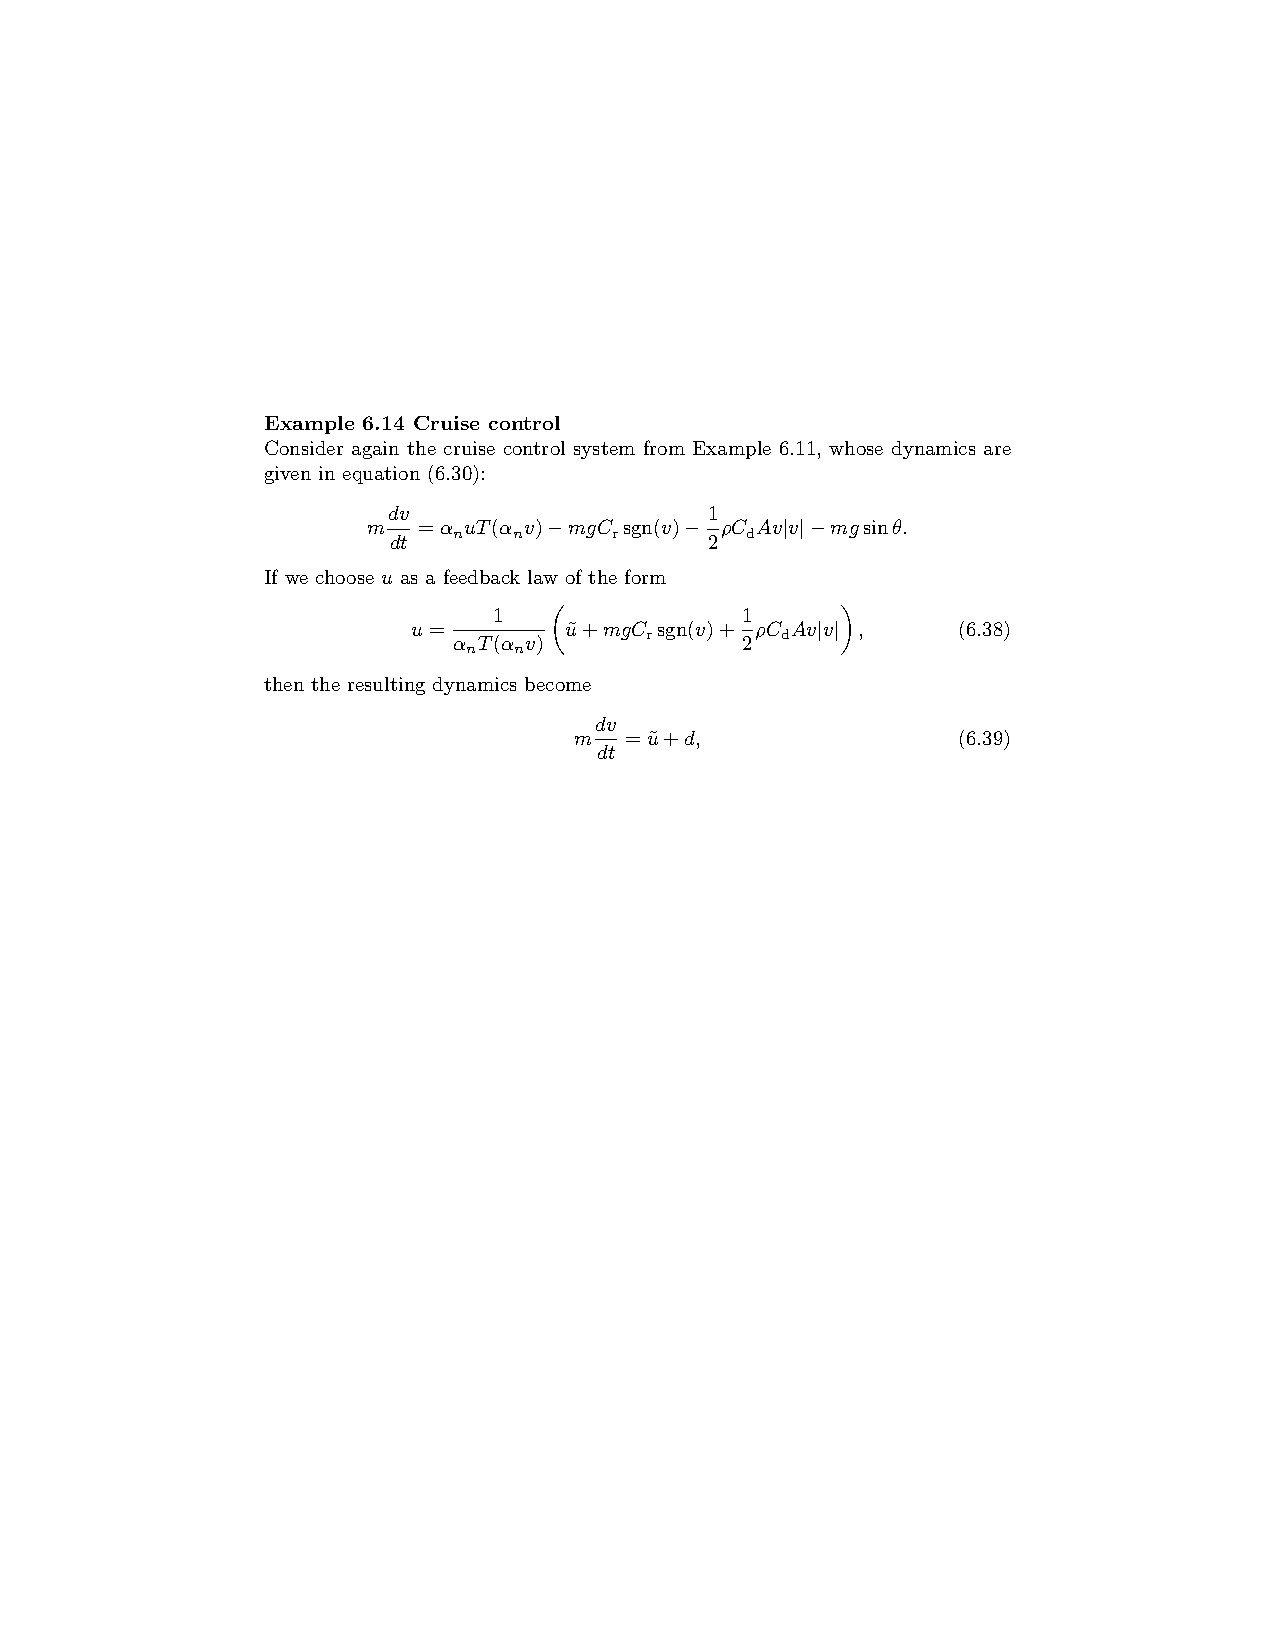
\includegraphics[width=\linewidth]{example6.14}

\end{frame}

\begin{frame}
\frametitle{Block diagram of feedback linearisation}
\centering

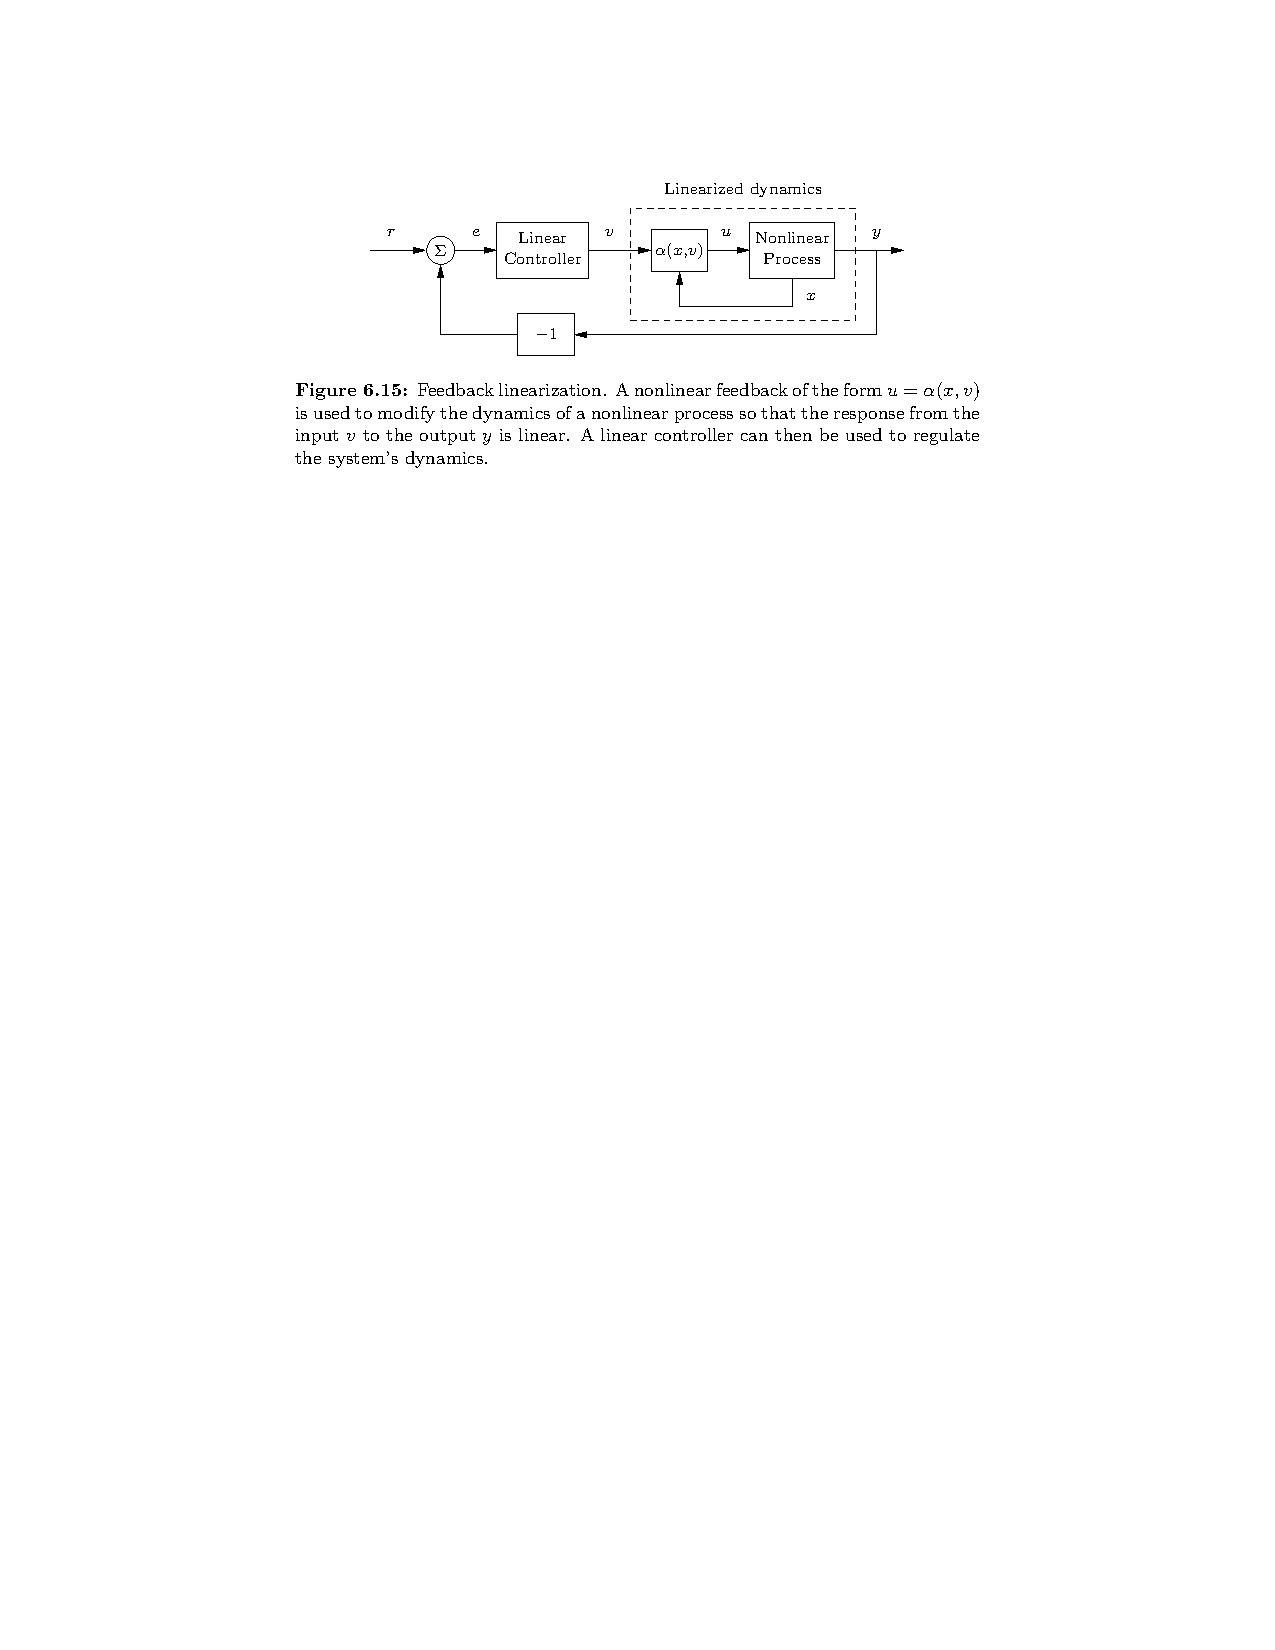
\includegraphics[width=\linewidth]{figure6.15}

\end{frame}

\begin{frame}
\frametitle{Dynamic inversion}
Generalised mechanical system with $M(q)$, $C(q,\dot q)$, $B(q)$:
\begin{align}
M(q)\ddot q + C(q,\dot q) = B(q) u \\
u = B(q)^{-1} \left( M(q) \alert{v} + C(q,\dot q) \right)
\end{align}
Resulting dynamics of the system are:
\begin{align}
M(q)\ddot q &= M(q) \alert{v} & \therefore\qquad \ddot q &= v
\end{align}
All dynamics are cancelled, assuming we can model them accurately and the actuators can react appropriately
\end{frame}

\SUMMARYFRAME
\FINALE

\end{document}
